\section{Usability Analyse}

Zuerst soll eine Analyse der IST-Situation, also der Android - Applikation, Aufschluss dar"uber geben, was Positiv ist und wo Verbesserungen an der Usability angebracht sind. 

\subsection{IST - Stand}
Der Aktuelle Stand ist eine Android Applikation, die  vom Verhalten und von der Optik her, an die zus"atzlich entwickelte Webapplikation angelehnt ist, und Elemente anderer bekannter mobiler Applikationen aufgreift um die geplanten Funktionen umzusetzen. 

Anhand verschiedener Screenshots soll im folgenden dargestellt werden was positiv/ negativ ist  und welche L"osungen als Verbesserungen umgesetzt werden k"onnten. 

\subsubsection{Login}
\begin{figure}[h]
 
\begin{subfigure}{0.5\textwidth}
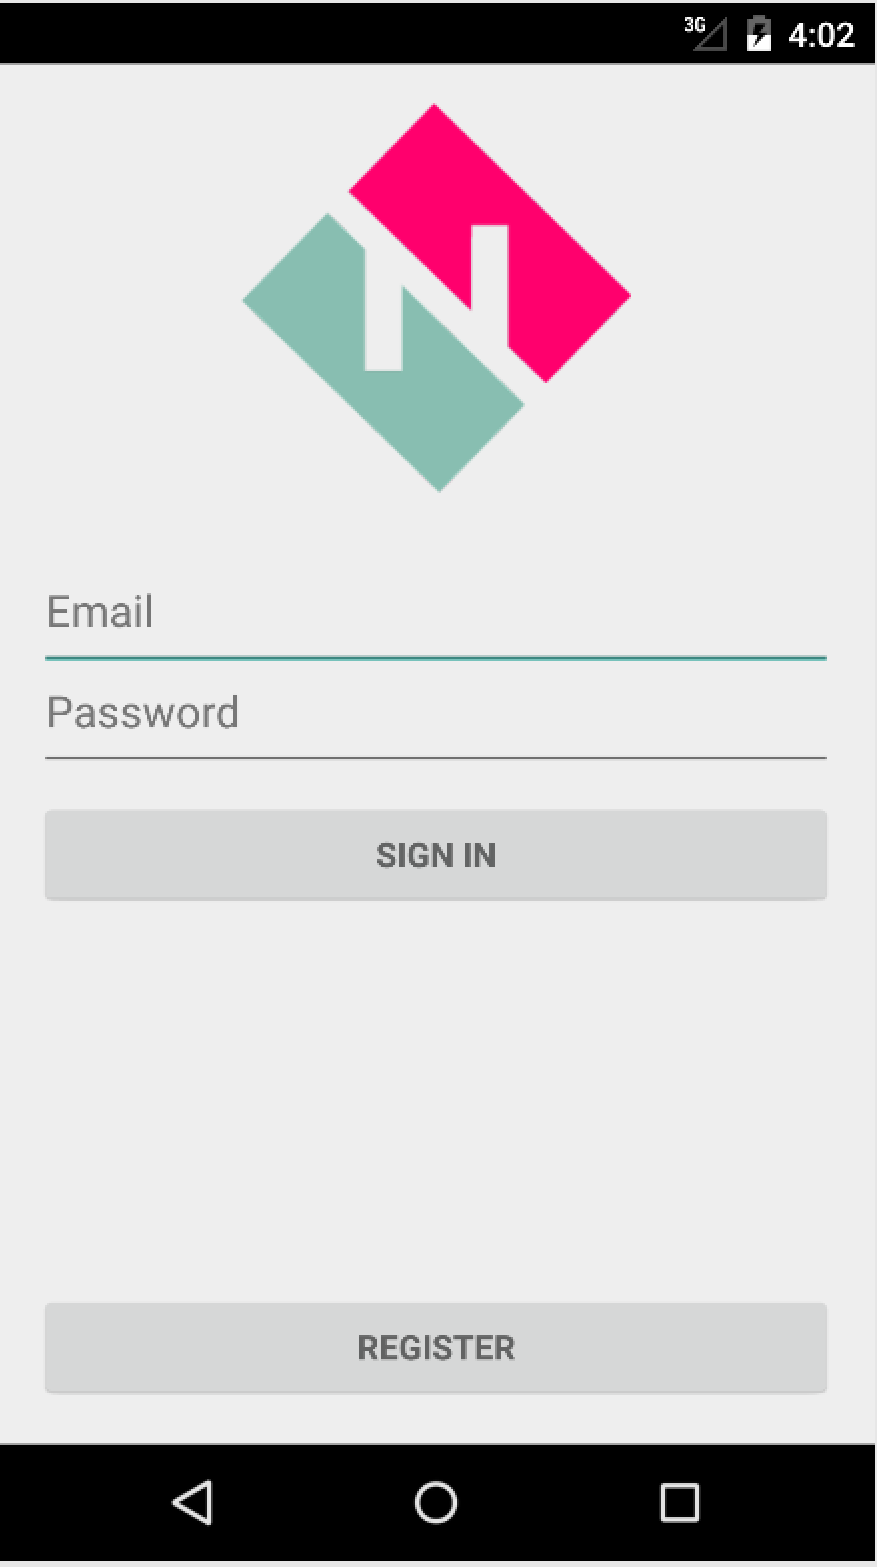
\includegraphics[width=0.9\linewidth]{./Bilder/logIn.png} 
\caption{LogIn Screen}
\label{fig:login}
\end{subfigure}
\begin{subfigure}{0.5\textwidth}
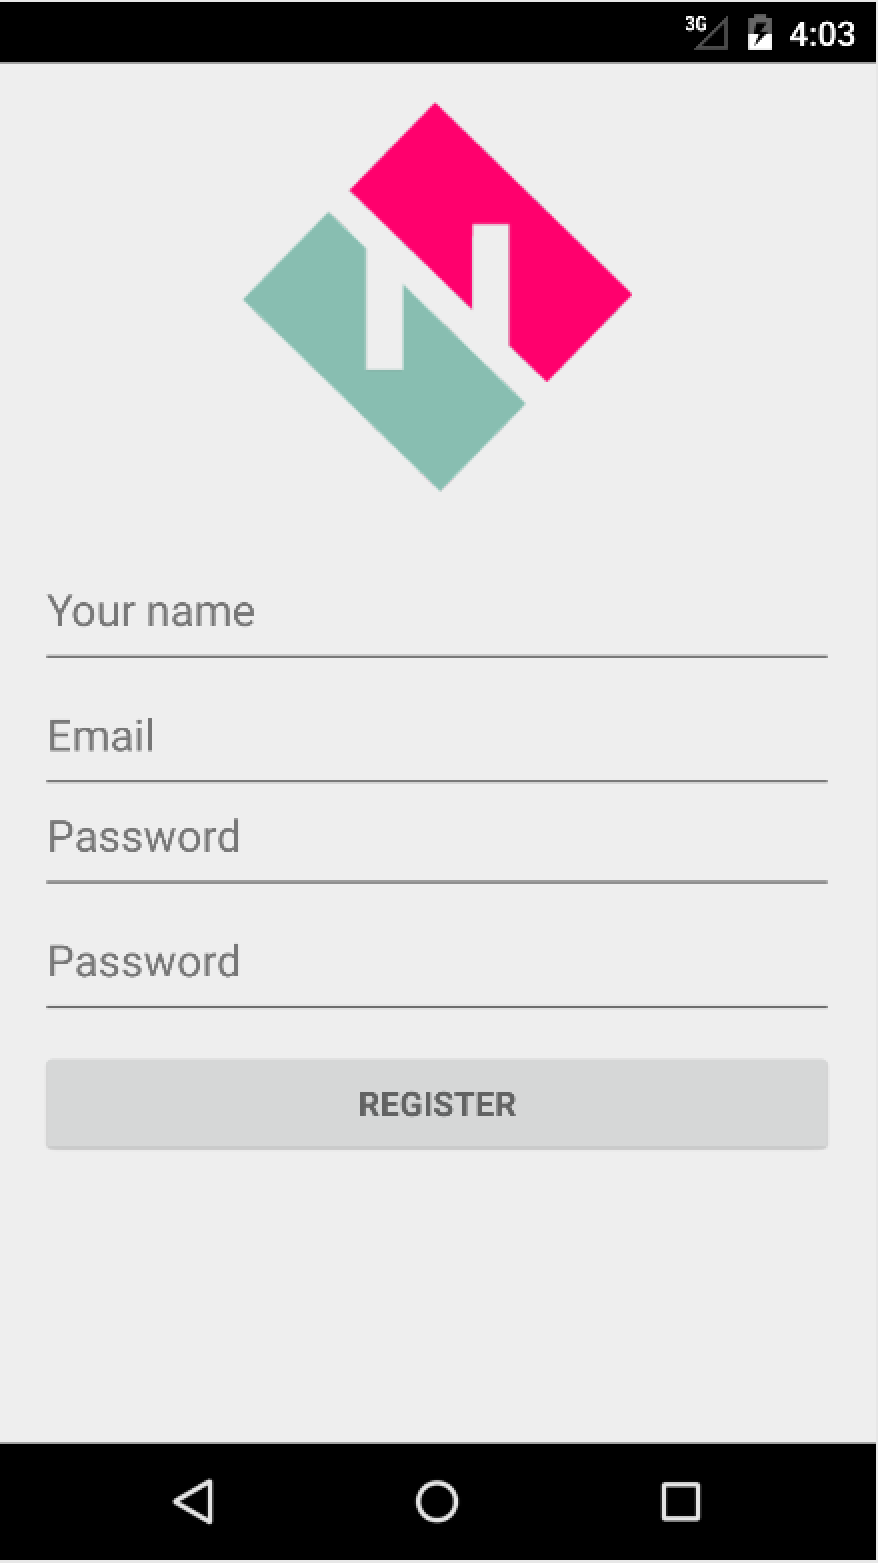
\includegraphics[width=0.9\linewidth]{./Bilder/signUp.png}
\caption{SignUp Screen}
\label{fig:signin}
\end{subfigure}
\caption{}
\label{fig:image2}
\end{figure}

 Startet man die ab findet man sich zuerst auf einem LogIn/SignUp - Screen wieder. 
 Hier kann durch die Eingabe einer g"ultigen Email-adresse und eines Passworts ein Account erstellt, oder sich in einen bestehenden Account eingeloggt werden. 
 Die Umsetzung ist schlicht und funktional gehalten. 
 Dies kann so "ubernommen werden. 
 
 Was erst im Vergleich mit den folgenden Seiten auff"allt, ist dass das Design dieser Seite nicht in das Schema der restlichen App passt. 
 Aus Gr"unden der Konsistenz wird das angepasst 
  
\subsubsection{Start}
\begin{figure}[h]
\begin{center}
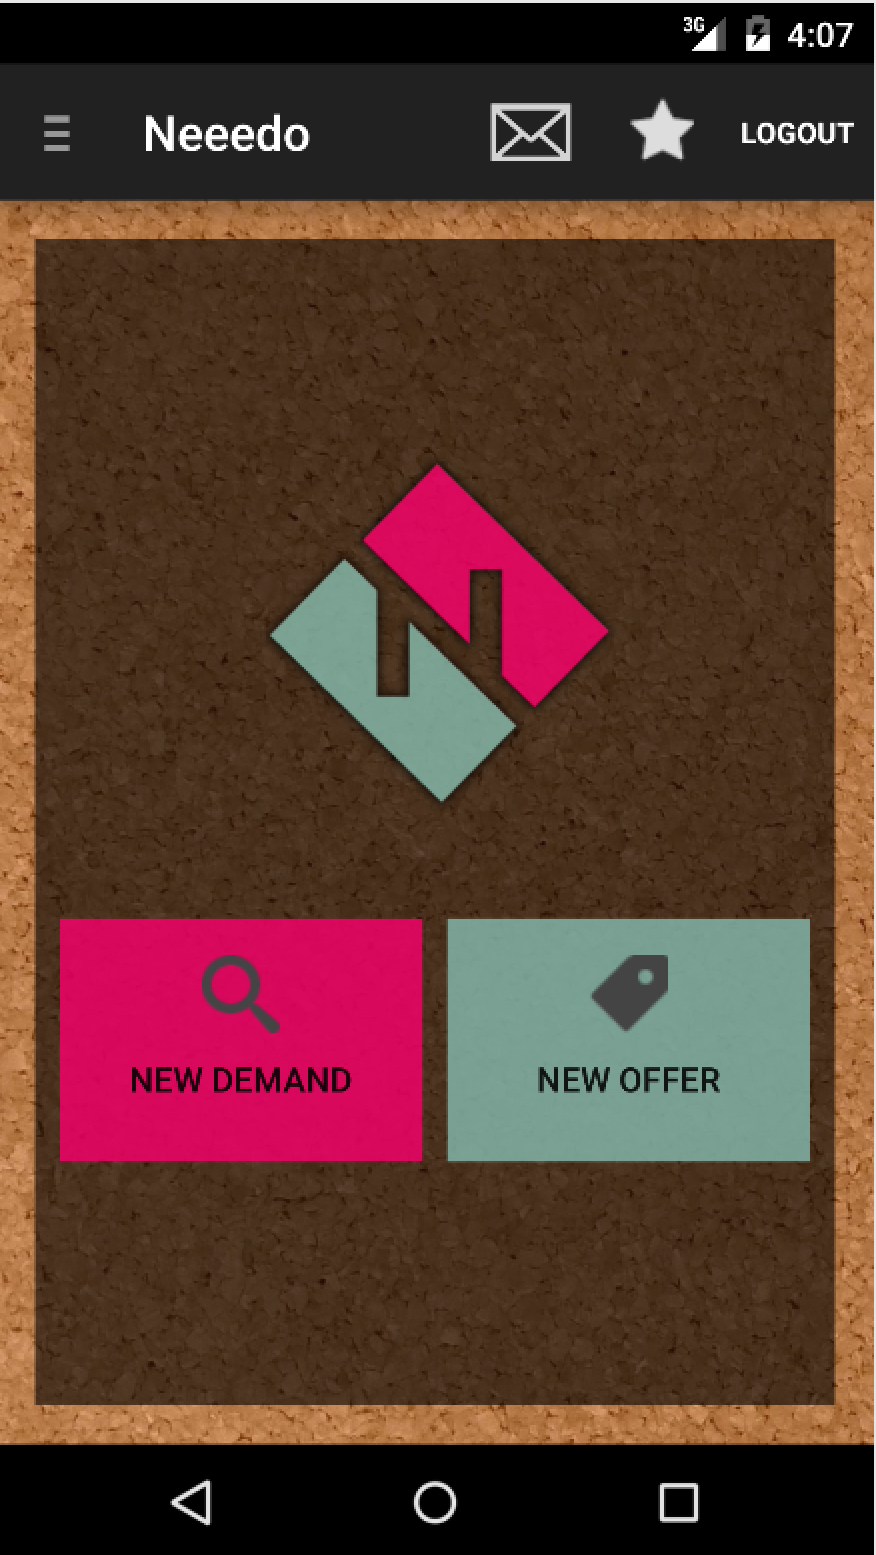
\includegraphics[width=0.45\textwidth]{./Bilder/start.png}
\caption{LandingScreen}
\label{fig:start}
\end{center}
\end{figure}

Loggt man sich ein landet man auf der hier abgebildeten LandingPage. 
Diese ist schlicht gehalten, jedoch ist nicht sofort ersichtlich was man hier tun soll. 
Auf dem halbtransparenten Hintergrund finden sich zwei Button, \enquote{New Demand} und \enquote{New Offer}, die einen wohl zu den Formularen f"uhren mit denen man diese erstellen kann. 
Man sieht am oberen Rand des Screens eine Men"uleiste, die einen "BurgerButton" als Men"u, den Schriftzug "Neeedo", ein Briefsymbol als Hinweis auf Nachrichten und einen Logout-Button beinhaltet. 
Dies ist eine (Android-) typische Positionierung f"ur diese  Elemente. 

Der Men"u Button ist dabei der am wenigsten markante, obwohl man wohl davon ausgehen kann, dass er der wichtigste ist. 
Dieser m"usste markanter sein. 

\subsubsection{Men"u}
\begin{figure}[h]
\begin{center}
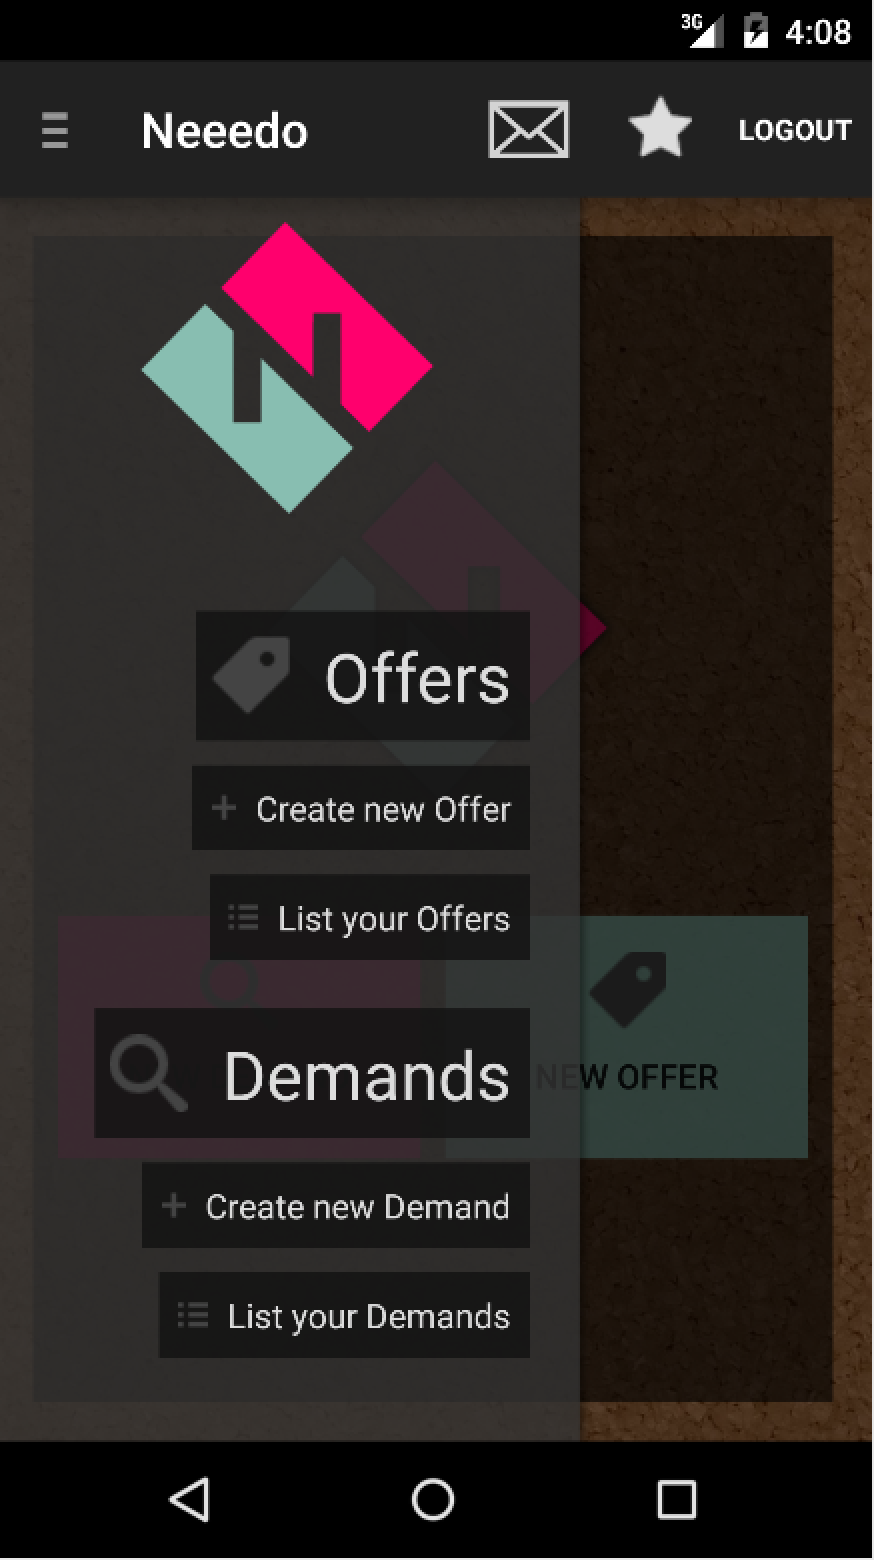
\includegraphics[width=0.45\textwidth]{./Bilder/menu.png}
\caption{Men"u offen}
\label{fig:menu}
\end{center}
\end{figure}

Benutzt man den \enquote{Men"u-Button} "offnet sich das hier abgebildete Men"u.
Diese bietet, vier Funktionen an: \enquote{Neues Gesuch erstellen}, \enquote{Neues Angebot erstellen}, \enquote{Eigene Angebote auflisten}, \enquote{Eigene Gesuche auflisten}.

Die Umrandung um die Worte, hier, \enquote{Offers} und \enquote{Demands} l"asst vermuten, dass es sich hierbei um Buttons handelt. 
Dies ist nicht der Fall. 
Es handelt sich hierbei nur um Trenner, die das Men"u in drei Sektionen unterteilt. 

Betrachtet man sich das Men"u als ganzes f"allt auf, dass es viel zu viel Platz einnimmt und unn"otig scheint. 
Um ein solches Men"u zu rechtfertigen m"ssten mehr Funktionen angeboten werden. 

\subsubsection{Agebote und Gesuche erstellen }
\begin{figure}[H]
\begin{subfigure}{0.5\textwidth}
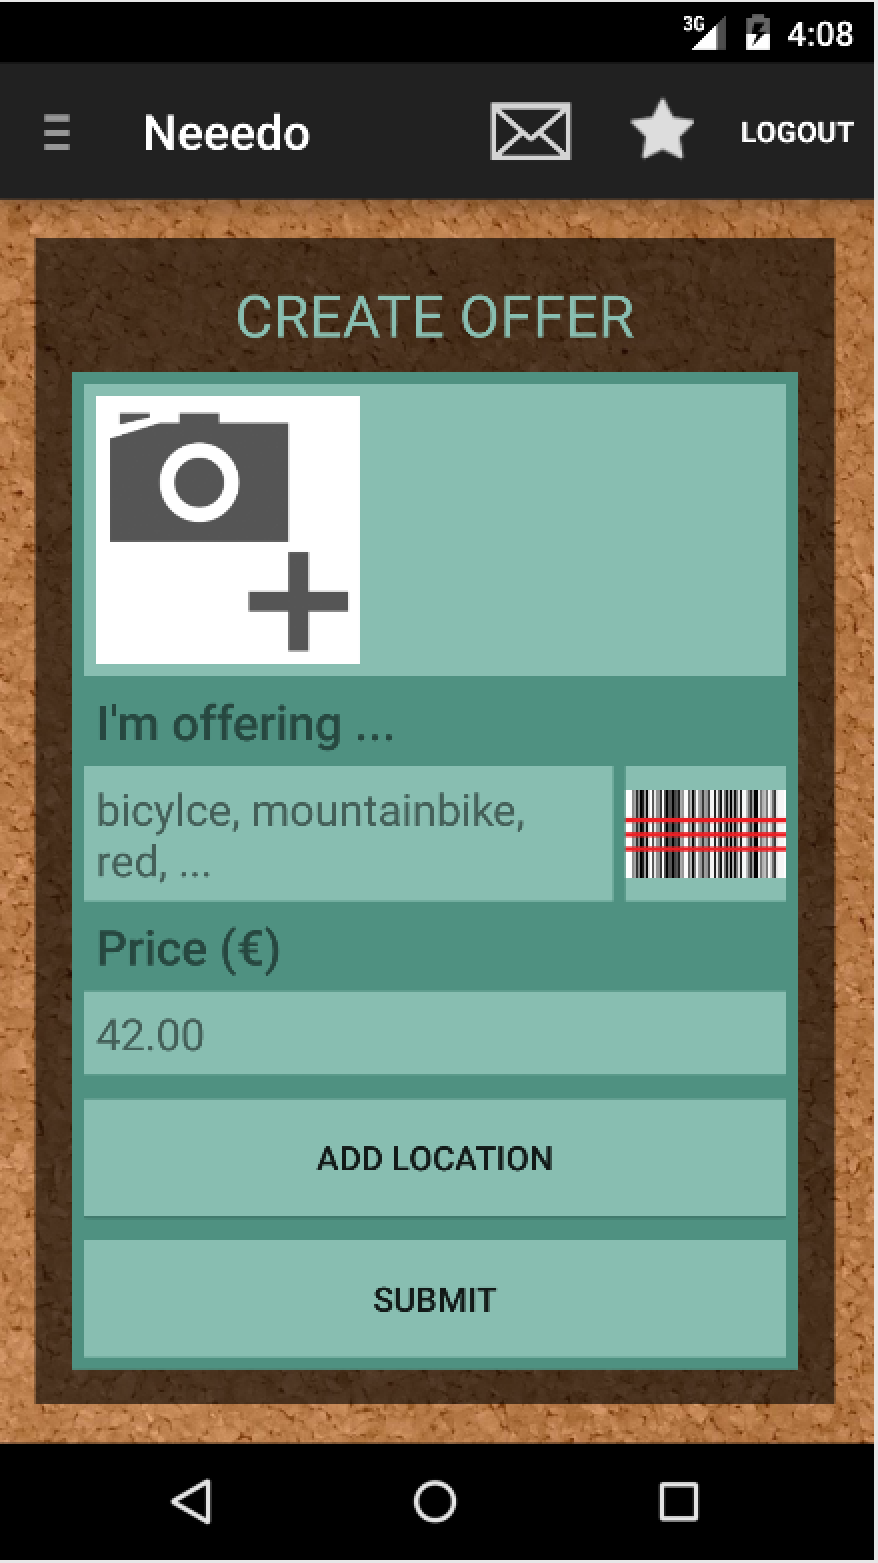
\includegraphics[width=0.9\linewidth]{./Bilder/createOffer.png} 
\caption{Angebot erstellen}
\label{fig:offer}
\end{subfigure}
\begin{subfigure}{0.5\textwidth}
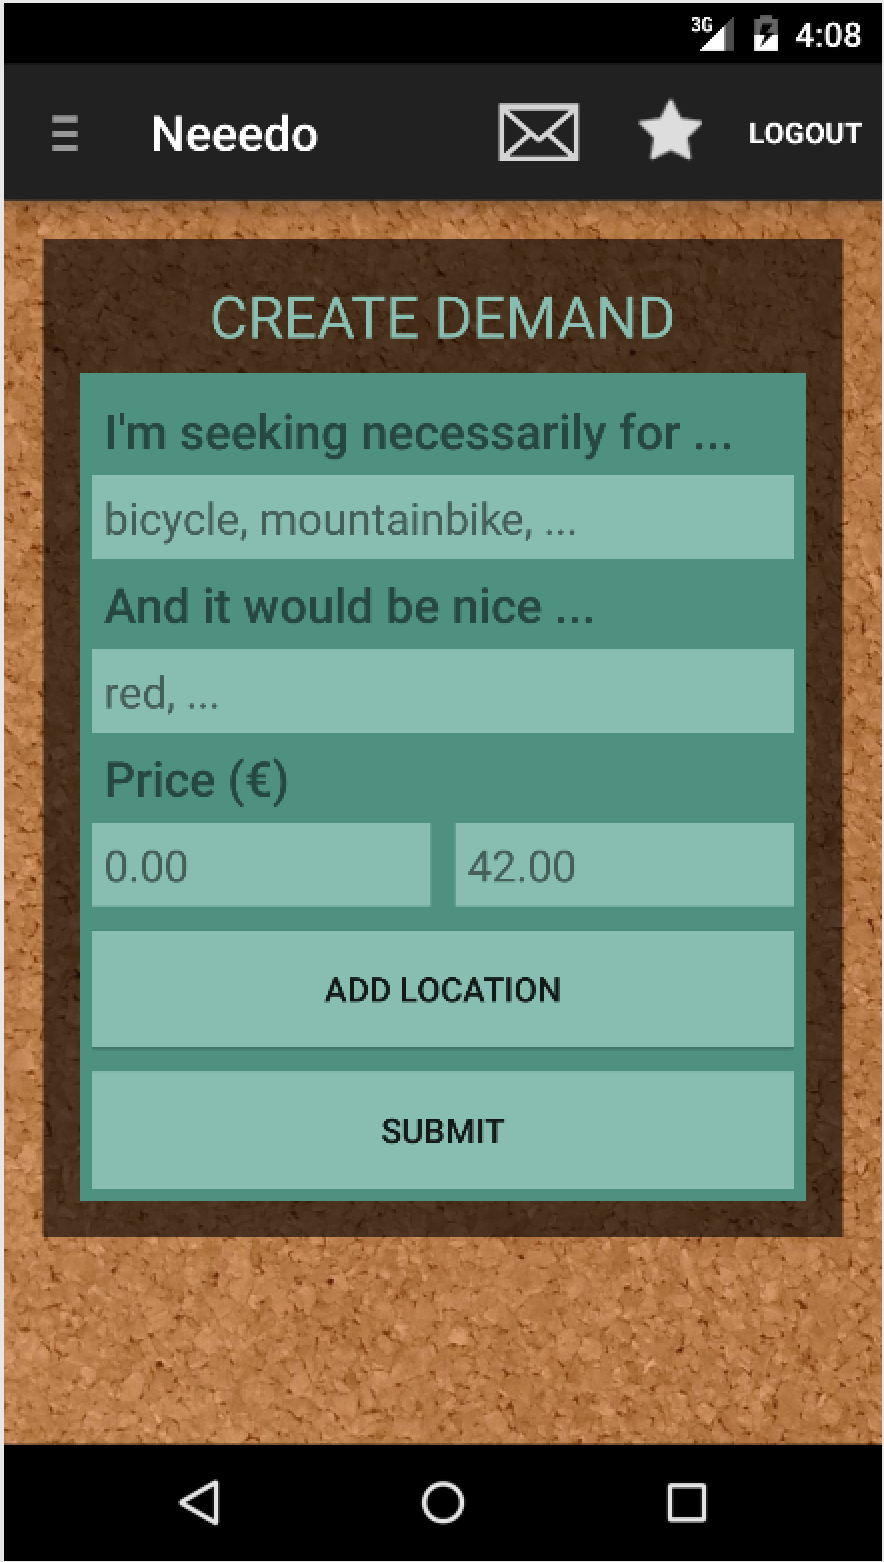
\includegraphics[width=0.9\linewidth]{./Bilder/createDemand.png}
\caption{Gesuch erstellen}
\label{fig:demand}
\end{subfigure}
\caption{}
\label{fig:image4}
\end{figure}

W"ahlt man entweder im Men"u oder auf dem StartScreen eine der Erstellfunktionen aus, landet man auf einer dieser Seiten entsprechend der Auswahl.
Hier wird jeweils ein Formular angezeigt, in dem man eintragen kann was man sucht oder was man anbieten m"ochte. 

Erstellt man ein Angebot/Offer ist es m"oglich Fotos zu hinzuzuf"ugen. 
Dies geschieht durch Auswahl des Camera-Bildes. Dieses ist nicht auf den ersten Blick als Button erkennbar. 
Ebenfalls erh"allt man die M"oglichkeit informationen "uber sein Produkt durch das Scannen eines Barcodes zu erhalten. 
Diese Funktionen sind sinnvoll und k"onnten in "ahnlicher Weise "ubernommen werden.

Erstellt man ein Gesuch/Demand, hat man weniger M"oglichkeiten zur Unterst"utzung. 
Hier muss schlicht das Formular ausgef"ullt werden

Beide Formulare besitzen die M"oglichkeit eine Adresse hinzuzuf"ugen, dies geschieht auf einer weiteren Seite, auf der dies durch Auswahl einer Positon auf einer Karte geschieht.

Es ist hier nicht klar erkennbar ob die Eingabe einer Position wirklich n"otig ist, oder was der Standardwert w"are.
 
\subsubsection{Matching}
\begin{figure}[H]
 
\begin{subfigure}{0.5\textwidth}
\includegraphics[width=0.9\linewidth]{./Bilder/matching1.png} 
\caption{Angebot erstellen}
\label{fig:match1}
\end{subfigure}
\begin{subfigure}{0.5\textwidth}
\includegraphics[width=0.9\linewidth]{./Bilder/matching2.png}
\caption{Gesuch erstellen}
\label{fig:match2}
\end{subfigure}
\caption{}
\label{fig:image5}
\end{figure}

Sendet man das Gesuch erstellen Formular ab wird man auf diese \enquote{Matching-View} weitergeleitet. 
Hier werden einem in einer, u.a. aus der App "Tinder" bekannten Stapel-Darstellung passende Angebote pr"sentiert. Diese k"onnen entweder durch die Buttons oder durch eine Swipe-Geste nach rechts oder Links verworfen oder als Favorite gespeichert werden. 
Um die gespeicherten Favoriten aufzurufen muss man den Stern in der Men"uleiste nutzen, im Screen selbst ist keine Weiterleitung m"oglich. 

\subsubsection{Eigene anzeigen}

\begin{figure}[h]
\begin{center}
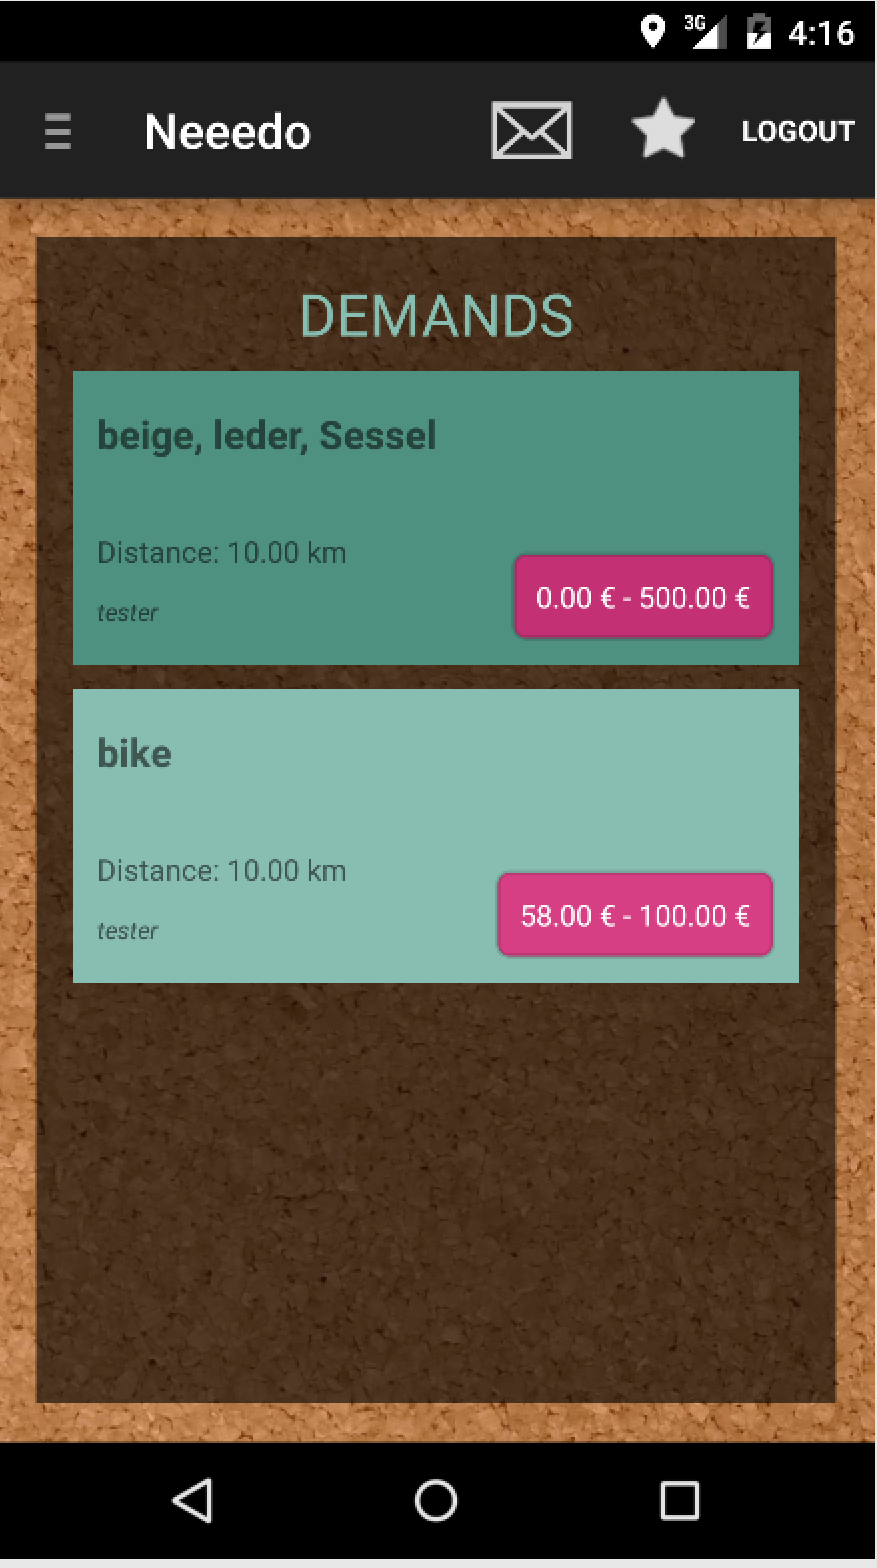
\includegraphics[width=0.45\textwidth]{./Bilder/liste.png}
\caption{Eigene Demands anzeigen}
\label{fig:anzeigen}
\end{center}
\end{figure}

Im Men"u finden sich auch die Funktionen \enquote{eigene Angebote/Gesuche anzeigen}. 
Benutzt man einen dieser Buttons, wird eine Tabelle wie die hier abgebildet pr"asentiert.
Klickt man hier auf eines der aufgef"uhrten Elemente, wird man auf ein Formular "ahnlich dem des Erstellens geleitet, auf dem "Anderungen durchgef"uhrt werden k"onnen. 


\subsection{Fazit}

Dies sind die wichtigsten Funktionen dieser App, weitere wie der Versand von Nachrichten werden nicht n"aher betrachtet, da hier nur ein Standard Chat zum Einsatz kommt. 

\subsubsection{Positiv}\begin{description}
\item[+] Das Design ist einheitlich 
\item[+] 
\end{description}

\subsubsection{Negativ}\begin{description}
\item[-] Nicht alle Buttons k"onnen als solche erkannt werden
\item[-] Elemente k"onnen irrt"umlich f"ur Buttons gehalten werden.
\item[-] Seitenmen"u zu gro"s und unpraktisch 
\item[-] Login nicht im selben Design
\end{description}

